
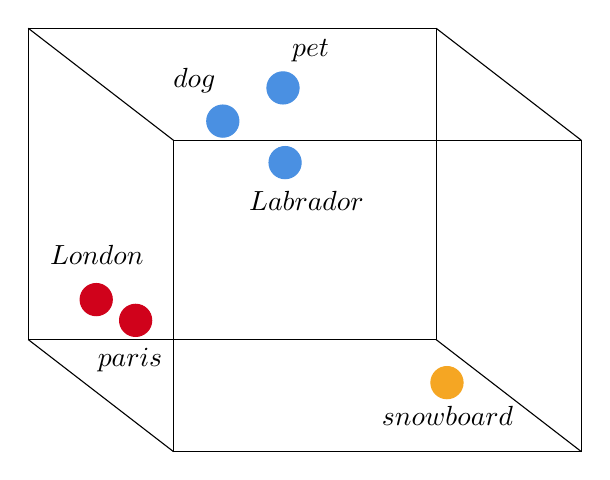
\begin{tikzpicture}[x=0.75pt,y=0.75pt,yscale=-1,xscale=1]
%uncomment if require: \path (0,300); %set diagram left start at 0, and has height of 300

%Shape: Rectangle [id:dp09766223150045761] 
\draw   (53,38) -- (249.5,38) -- (249.5,188) -- (53,188) -- cycle ;
%Shape: Rectangle [id:dp15444454726665247] 
\draw   (123,92) -- (319.5,92) -- (319.5,242) -- (123,242) -- cycle ;
%Straight Lines [id:da41180023590596115] 
\draw    (53,38) -- (123,92) ;


%Straight Lines [id:da8327746912035379] 
\draw    (53,188) -- (123,242) ;


%Straight Lines [id:da7076376732109662] 
\draw    (249.5,38) -- (319.5,92) ;


%Straight Lines [id:da531943191161679] 
\draw    (249.5,188) -- (319.5,242) ;


%Shape: Circle [id:dp5653236923369969] 
\draw  [color={rgb, 255:red, 74; green, 144; blue, 226 }  ,draw opacity=1 ][fill={rgb, 255:red, 74; green, 144; blue, 226 }  ,fill opacity=1 ] (168,66.75) .. controls (168,62.47) and (171.47,59) .. (175.75,59) .. controls (180.03,59) and (183.5,62.47) .. (183.5,66.75) .. controls (183.5,71.03) and (180.03,74.5) .. (175.75,74.5) .. controls (171.47,74.5) and (168,71.03) .. (168,66.75) -- cycle ;
%Shape: Circle [id:dp7862090364041379] 
\draw  [color={rgb, 255:red, 74; green, 144; blue, 226 }  ,draw opacity=1 ][fill={rgb, 255:red, 74; green, 144; blue, 226 }  ,fill opacity=1 ] (169,102.75) .. controls (169,98.47) and (172.47,95) .. (176.75,95) .. controls (181.03,95) and (184.5,98.47) .. (184.5,102.75) .. controls (184.5,107.03) and (181.03,110.5) .. (176.75,110.5) .. controls (172.47,110.5) and (169,107.03) .. (169,102.75) -- cycle ;
%Shape: Circle [id:dp04017773076556641] 
\draw  [color={rgb, 255:red, 74; green, 144; blue, 226 }  ,draw opacity=1 ][fill={rgb, 255:red, 74; green, 144; blue, 226 }  ,fill opacity=1 ] (139,82.75) .. controls (139,78.47) and (142.47,75) .. (146.75,75) .. controls (151.03,75) and (154.5,78.47) .. (154.5,82.75) .. controls (154.5,87.03) and (151.03,90.5) .. (146.75,90.5) .. controls (142.47,90.5) and (139,87.03) .. (139,82.75) -- cycle ;
%Shape: Circle [id:dp3593472220907403] 
\draw  [color={rgb, 255:red, 245; green, 166; blue, 35 }  ,draw opacity=1 ][fill={rgb, 255:red, 245; green, 166; blue, 35 }  ,fill opacity=1 ] (247,208.75) .. controls (247,204.47) and (250.47,201) .. (254.75,201) .. controls (259.03,201) and (262.5,204.47) .. (262.5,208.75) .. controls (262.5,213.03) and (259.03,216.5) .. (254.75,216.5) .. controls (250.47,216.5) and (247,213.03) .. (247,208.75) -- cycle ;
%Shape: Circle [id:dp42932079750070606] 
\draw  [color={rgb, 255:red, 208; green, 2; blue, 27 }  ,draw opacity=1 ][fill={rgb, 255:red, 208; green, 2; blue, 27 }  ,fill opacity=1 ] (78,168.75) .. controls (78,164.47) and (81.47,161) .. (85.75,161) .. controls (90.03,161) and (93.5,164.47) .. (93.5,168.75) .. controls (93.5,173.03) and (90.03,176.5) .. (85.75,176.5) .. controls (81.47,176.5) and (78,173.03) .. (78,168.75) -- cycle ;
%Shape: Circle [id:dp1106554795442356] 
\draw  [color={rgb, 255:red, 208; green, 2; blue, 27 }  ,draw opacity=1 ][fill={rgb, 255:red, 208; green, 2; blue, 27 }  ,fill opacity=1 ] (97,178.75) .. controls (97,174.47) and (100.47,171) .. (104.75,171) .. controls (109.03,171) and (112.5,174.47) .. (112.5,178.75) .. controls (112.5,183.03) and (109.03,186.5) .. (104.75,186.5) .. controls (100.47,186.5) and (97,183.03) .. (97,178.75) -- cycle ;

% Text Node
\draw (133,63) node   {$dog$};
% Text Node
\draw (189,49) node   {$pet$};
% Text Node
\draw (187,121) node   {$Labrador$};
% Text Node
\draw (255,225) node   {$snowboard$};
% Text Node
\draw (86,147) node   {$London$};
% Text Node
\draw (102,198) node   {$paris$};


\end{tikzpicture}


